\documentclass[usenames,dvipsnames]{beamer}

\usetheme{Madrid}
\usecolortheme{dolphin}
\setbeamercolor{title}{fg=NavyBlue}
\setbeamercolor{frametitle}{fg=NavyBlue}
\setbeamercolor{section in toc}{fg=NavyBlue}

\usepackage{amsthm}
\usepackage{graphicx}
\usepackage[utf8x]{inputenc}
\usepackage{mathtools,amssymb}
\mathtoolsset{showonlyrefs}
\usepackage{appendixnumberbeamer}
\usepackage{centernot}
\usepackage{tikz}
\usepackage[lined]{algorithm2e}
\usepackage{caption}
\usetikzlibrary{positioning}
\usepackage{booktabs}
\usepackage{natbib}
\usepackage{appendix}
\usepackage{perpage}
\MakePerPage{footnote}

% Itemize settings
\settowidth{\leftmargini}{\usebeamertemplate{itemize item}}
\addtolength{\leftmargini}{\labelsep}
\setbeamertemplate{itemize items}[default]
\setbeamertemplate{enumerate items}[default]

% Commands
\DeclarePairedDelimiter{\abs}{\lvert}{\rvert}
\DeclarePairedDelimiter{\norm}{\|}{\|}
\renewcommand{\Pr}{\mathbb{P}}
\newcommand{\R}{\mathbb{R}}
\newcommand{\Var}{\operatorname{Var}}
\newcommand{\E}{\operatorname{\mathbb{E}}}
\newcommand{\iid}{\ensuremath{\stackrel{\text{iid}}{\sim}}}
\renewcommand{\phi}{\varphi}
\newcommand{\epl}{\varepsilon}
\renewcommand{\d}{\mathrm{d}}
\newcommand{\dd}{\,\mathrm{d}}
\newcommand{\lratext}[1]{\ensuremath{\stackrel{\text{#1}}{\longrightarrow}}}
\newcommand{\toweak}{\rightharpoonup}

% Theorem blocks
\setbeamercolor{block title}{fg=white,bg=NavyBlue}
\newenvironment<>{greenblock}[1][]{%
\setbeamercolor{block title}{fg=white,bg=ForestGreen}%
\begin{block}#2{#1}}{\end{block}}
\newenvironment<>{redblock}[1][]{%
\setbeamercolor{block title}{fg=white,bg=red!75!black}%
\begin{block}#2{#1}}{\end{block}}
\newenvironment<>{orangeblock}[1][]{%
\setbeamercolor{block title}{fg=white,bg=orange!75!black}%
\begin{block}#2{#1}}{\end{block}}
\setbeamercolor{caption name}{fg=NavyBlue}

% Add numbers and take out navigation symbols
\beamertemplatenavigationsymbolsempty
\setbeamercolor{date in head/foot}{fg=gray, bg=white}
\setbeamercolor{author in head/foot}{fg=white,bg=white}
\setbeamercolor{title in head/foot}{fg=white,bg=white}
\setbeamertemplate{footline}{
	\leavevmode%
	\hbox{%
		\begin{beamercolorbox}[wd=.4\paperwidth,ht=2.25ex,dp=1ex,center]{author in head/foot}%
		\end{beamercolorbox}%
		\begin{beamercolorbox}[wd=.3\paperwidth,ht=2.25ex,dp=1ex,center]{title in head/foot}%
		\end{beamercolorbox}%
		\begin{beamercolorbox}[wd=.3\paperwidth,ht=2.25ex,dp=1ex,right]{date in head/foot}%
			\insertframenumber{} / \inserttotalframenumber\hspace*{2ex} 
	\end{beamercolorbox}}%
	\vskip0pt%
}

% Colors
\definecolor{leg1}{RGB}{0,114,189}
\definecolor{leg2}{RGB}{217,83,25}
\definecolor{leg3}{RGB}{237,177,32}
\definecolor{leg4}{RGB}{126,47,142}
\definecolor{leg5}{RGB}{119,172,48}
\newcommand{\FG}[1]{{\color{ForestGreen}#1}}
\newcommand{\NB}[1]{{\color{NavyBlue}#1}}
\newcommand{\BR}[1]{{\color{BrickRed}#1}}

% Text starts always from the top of the frame
\newenvironment{frameT}{\begin{frame}[t]}{\end{frame}}

\newcommand*\samethanks[1][\value{footnote}]{\footnotemark[#1]}
\title{A pre-processing technique for asymptotically correct drift estimation in multiscale diffusion processes}
\author{Assyr Abdulle \thanks{Institute of Mathematics, EPFL} \and Giacomo Garegnani \samethanks[1] \and Grigorios A. Pavliotis \thanks{Department of Mathematics, Imperial College London}  \\ \and Andrew M. Stuart \thanks{Department of Computing and Mathematical Sciences, Caltech} \and Andrea Zanoni \samethanks[1]}
\date{Imperial College London -- 7 February 2020}
\institute[EPFL]{École polytechnique fédérale de Lausanne \\ \vspace{0.5cm} 
\includegraphics[width=3cm]{Logo-eps-converted-to.pdf}}

%@unpublished{AGP20,
%	author = {Abdulle, A and Garegnani, G and Pavliotis, G A and Stuart, A M and Zanoni, A},
%	title = {Drift estimation of multiscale diffusions via filtering},
%	year = {2020},
%	note = {In preparation}
%}


\begin{document}

\thispagestyle{empty}
\frame{\titlepage}

\addtocounter{framenumber}{-1}

\begin{frame}
\frametitle{Setting - Homogenization}

	\only<1>{
	\BR{Multiscale SDE}
	}
	\only<1-2>{
	\begin{equation}
		\d X_t^\epl = -\alpha \cdot V'(X_t^\epl) \dd t - \frac1\epl p'\left(\frac{X_t^\epl}\epl\right) \dd t+ \sqrt{2\sigma} \dd W_t.
	\end{equation}
	}
	\only<1>{
		
	\vspace{0.1cm}
	\NB{Parameters}:
	\begin{itemize}
		\item drift coefficient $\alpha \in \R^N$ 
		\item slow potential $V\colon \R \to \R^N$, $V(x) = (V_1(x), V_2(x), \ldots, V_N(x))^\top$,
		\item fast potential $p\colon \R \to \R$, $L$-periodic
		\item diffusion coefficient $\sigma > 0$
		\item multiscale parameter $\epl > 0$
		\item standard one-dimensional BM $W_t$
	\end{itemize}
	}
	\only<2>{
	
	\vspace{0.1cm}
	\FG{Homogenization theory}: $X_t^\epl \to X_t$ in law for $\epl \to 0$ and
	\begin{equation}
		\d X_t = -A \cdot V'(X_t) \dd t + \sqrt{2\Sigma} \dd W_t,
	\end{equation}
	with $A = K\alpha$, $\Sigma = K\sigma$ and 
	\begin{equation}
		K = \int_0^L \left(1 + \Phi'(y)\right)^2  \mu(\d y), \quad \mu(\d y) = \frac1Z e^{-p(y)/\sigma} \dd y,
	\end{equation}
	with $\Phi$ solution of
	\begin{equation}
		-p'(y)\Phi'(y)+\sigma \Phi''(y) = p'(y), \quad 0 \leq y \leq L.
	\end{equation}
	}
\end{frame}

\begin{frame}
\frametitle{Setting - Parameter inference}

  	\onslide<1->{
  	\begin{equation}
	\begin{alignedat}{2}		
		&\BR{\d X_t^\epl = -\alpha \cdot V'(X_t^\epl) \dd t - \frac1\epl p'\left(\frac{X_t^\epl}\epl\right) \dd t+ \sqrt{2\sigma} \dd W_t } &&\quad \to \text{data} \\
  		&\FG{\d X_t = -A \cdot V'(X_t) \dd t + \sqrt{2\Sigma} \dd W_t} &&\quad \to \text{model}
	\end{alignedat}
	\end{equation}
	
	\vspace{0.2cm}
	\NB{Goal}: Estimate \FG{$A\in \R^N$} from observations \BR{$X^\epl = (X_t^\epl, 0\leq t\leq T)$}
	}	

	\vspace{0.2cm}
	\begin{overlayarea}{\textwidth}{0.5\textheight}
	\only<2>{	
	\NB{What we know}: 
	\begin{itemize}
		\item slow potential $V$ (i.e., $V'$)
	\end{itemize}

	\vspace{0.2cm}
	\NB{What we ignore}:
	\begin{itemize}
		\item the rest
	\end{itemize}
	}
	
	\only<3>{
	\NB{Idea}: Maximize likelihood function (Girsanov)
	\begin{align}
		L(X^\epl \mid A) &= \exp\left(-\frac{I(X^\epl \mid A)}{2\Sigma}\right), \\
		I(X^\epl \mid A) &= \int_0^T A \cdot V'(X^\epl_t) \dd X^\epl_t + \frac12 \int_0^T \left( A \cdot V'(X^\epl_t) \right)^2 \dd t.
	\end{align}
	}
	
	\only<4-5>{
		\NB{Idea}: Maximize likelihood function (Girsanov)
		\begin{equation}
		I(X^\epl \mid A) = \int_0^T A \cdot V'(X^\epl_t) \dd X^\epl_t + \frac12 \int_0^T \left( A \cdot V'(X^\epl_t) \right)^2 \dd t,
		\end{equation}
	}

	\only<4>{
		\NB{Estimator}:
		\begin{equation}
		\widehat A^\epl(T) = \vphantom{\left(\int_0^T V'(X^\epl_t) \otimes V'(X^\epl_t) \dd t\right)^{-1}\int_0^T V'(X^\epl_t) \dd X_t}{\arg \min_{A\in\R^N}I(X^\epl \mid A)},
		\end{equation}
	}

	\only<5>{
		\NB{Estimator}:
		\begin{equation}
			\widehat A^\epl(T) = \left(\int_0^T V'(X^\epl_t) \otimes V'(X^\epl_t) \dd t\right)^{-1}\int_0^T V'(X^\epl_t) \dd X^\epl_t,
		\end{equation}
	}

	\only<6>{
		\NB{Idea}: Maximize likelihood function (Girsanov)
		\begin{equation}
			I(X^\epl \mid A) = \int_0^T A V'(X^\epl_t) \dd X^\epl_t + \frac12 \int_0^T \left( A  V'(X^\epl_t) \right)^2 \dd t,
		\end{equation}
		\NB{Estimator}:
		\begin{equation}
			\widehat A^\epl(T) = - \frac{\int_0^T V'(X^\epl_t) \dd X^\epl_t}{\int_0^T V'(X^\epl_t)^2 \dd t}, \qquad (N = 1).
		\end{equation}
	}

	\only<7->{
		\NB{Estimator}:
		\begin{equation}
		\widehat A^\epl(T) = - \frac{\int_0^T V'(X^\epl_t) \dd X^\epl_t}{\int_0^T V'(X^\epl_t)^2 \dd t},
		\end{equation}
	}

	\only<7>{	
		\NB{Homogenization}: We have $X_t^\epl \to X_t$ for $\epl \to 0$
		\begin{equation}
			\implies \lim_{\epl \to 0}\lim_{T\to\infty} \widehat A^\epl(T) = A, \qquad \BR{\text{Wrong!}}
		\end{equation}
	}
	
	\only<8>{
		\NB{Homogenization}: We have $X_t^\epl \to X_t$ for $\epl \to 0$ \footnotemark
		\begin{equation}
			\implies \lim_{\epl \to 0}\lim_{T\to\infty} \widehat A^\epl(T) = \alpha, \qquad \BR{\text{Problem!}}
		\end{equation}
	}
	\end{overlayarea}
	\only<8>{\footnotetext{\cite{PaS07}}}
\end{frame}

\begin{frame}
	\frametitle{Solutions -- Literature}
	
	\begin{itemize}
		\item Subsample the data
		\begin{itemize}
			\item Theory: \cite{PaS07, PPS09}
			\item Practice: \cite{CoP09} (oceanography) \cite{ZMA05,OSP10,AiJ14} (econometrics) 
		\end{itemize}
		\item Martingale property-based
		\begin{itemize}
			\item Theory: \cite{KKP15, KPK13}
			\item Practice: \cite{KPP15}
		\end{itemize}
		\item Nonparameteric / Bayesian: \cite{PSV09, PSZ13} (single scale)
		\item \ldots
	\end{itemize}
\end{frame}

\begin{frame}
\frametitle{Subsampling the data}

	\only<1>{
		\NB{Estimator}:
		\begin{equation}
			\widehat A^\epl(T) = - \frac{\int_0^T V'(X^\epl_t) \dd X^\epl_t}{\int_0^T V'(X^\epl_t)^2 \dd t}.
		\end{equation}
		
		\BR{Problem}: $\lim_{\epl \to 0}\lim_{T\to\infty} \widehat A^\epl(T) \to \alpha$.
		
		\vspace{0.4cm}
		\FG{Solution}\footnote{\cite{PaS07}}: Subsample the data with step $\delta$ and compute
		\begin{equation}
			\widehat A^\epl_\delta(T) = - \frac{\sum_{i=0}^{N-1} V'(X^\epl_{i\delta}) \left(X^\epl_{(i+1)\delta}-X^\epl_{i\delta}\right)}{\delta \sum_{i=0}^{N-1}V'(X^\epl_{i\delta})^2}, \qquad N\delta = T.
		\end{equation}
	}
	
	\only<2>{
		\FG{Solution}\footnote{\cite{PaS07}}: Subsample the data with step $\delta$ and compute
		\begin{equation}
		\widehat A^\epl_\delta(T) = - \frac{\sum_{i=0}^{N-1} V'(X^\epl_{i\delta}) \left(X^\epl_{(i+1)\delta}-X^\epl_{i\delta}\right)}{\delta \sum_{i=0}^{N-1}V'(X^\epl_{i\delta})^2}, \qquad N\delta = T.
		\end{equation}
		
		\begin{theorem} If $\delta = \epl^\zeta$, $0<\zeta<1$ and $N = \lceil\epl^{-\gamma}\rceil$ with $\gamma > \zeta$, then
			\begin{equation}
			\lim_{\epl \to 0} \widehat A^\epl_\delta(T) = A, \quad {\text{in probability}}.
			\end{equation}
		\end{theorem}
		
		\vspace{0.2cm}
		\BR{Issue}: How do we choose $\zeta \in (0, 1)$?
	}
	
	\only<3>{
		\FG{Solution}\footnote{\cite{PaS07}}: Subsample the data with step $\delta$ and compute
		\begin{equation}
		\widehat A^\epl_\delta(T) = - \frac{\sum_{i=0}^{N-1} V'(X^\epl_{i\delta}) \left(X^\epl_{(i+1)\delta}-X^\epl_{i\delta}\right)}{\delta \sum_{i=0}^{N-1}V'(X^\epl_{i\delta})^2}, \qquad N\delta = T.
		\end{equation}
		
		\begin{theorem} If $\delta = \epl^\zeta$, $0<\zeta<1$ and $N = \lceil\epl^{-\gamma}\rceil$ with $\gamma > \zeta$, then
			\begin{equation}
				\lim_{\epl \to 0} \widehat A^\epl_\delta(T) = A, \quad {\text{in probability}}.
			\end{equation}
		\end{theorem}
	
		\vspace{0.2cm}
		\BR{Issue}: Take $\epl=0.1$, data $\tilde \delta = 0.01$, $\delta = \sqrt{\epl}\approx 0.3$ $\implies$ $97\%$ ``garbage''
	}

	\only<4>{
		\BR{Experiment}: Estimate $A$ for $V(x) = x^2/2$ (Ornstein--Uhlenbeck) with subsampling varying $\delta = \epl^\zeta$ ($\epl = 0.1$, $T = 10^3$, $p(y) = \cos(y)$)
		
		\begin{figure}
		\begin{tabular}{ccc}
			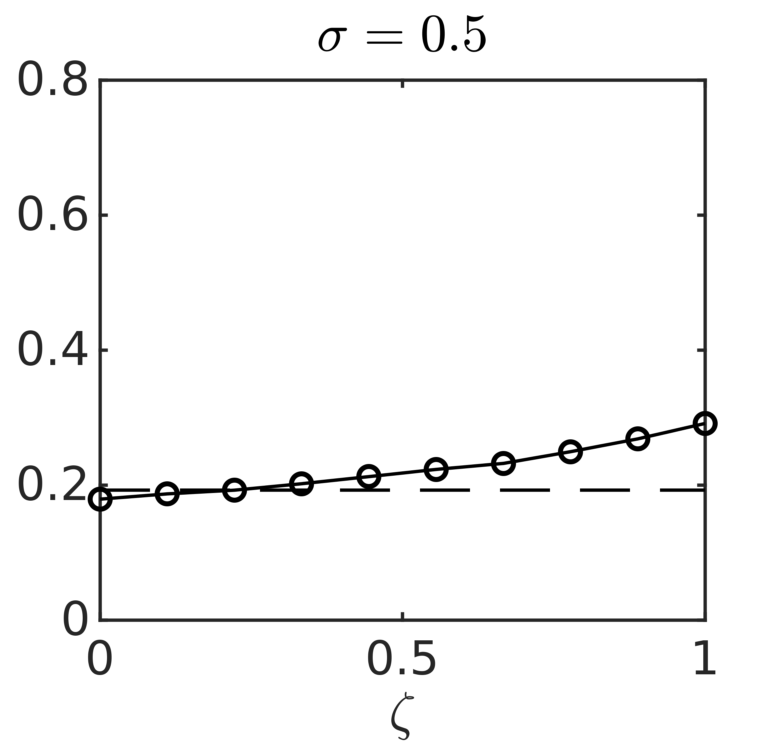
\includegraphics[scale=0.9]{Figures/OUSubs_s5} & 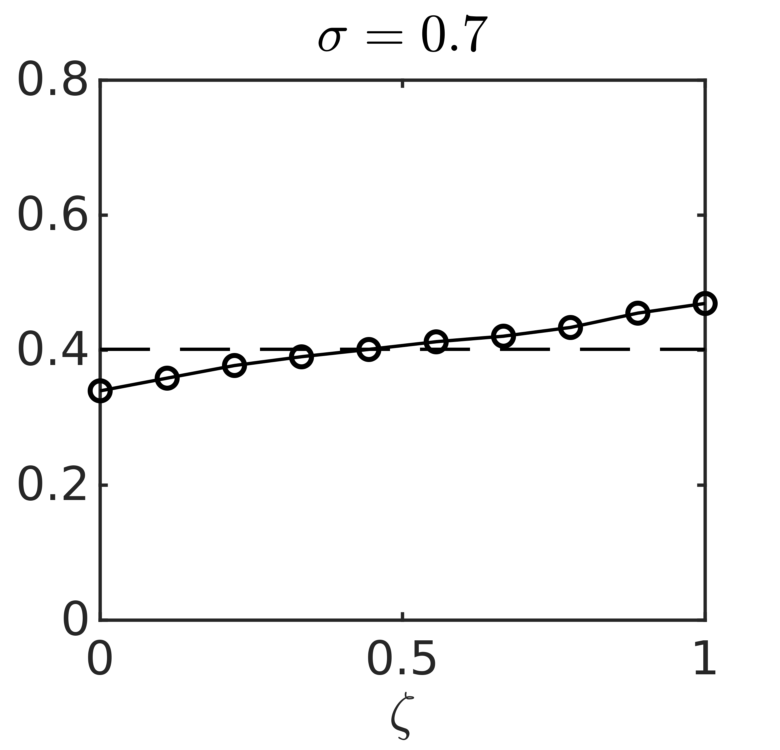
\includegraphics[scale=0.9]{Figures/OUSubs_s7} & 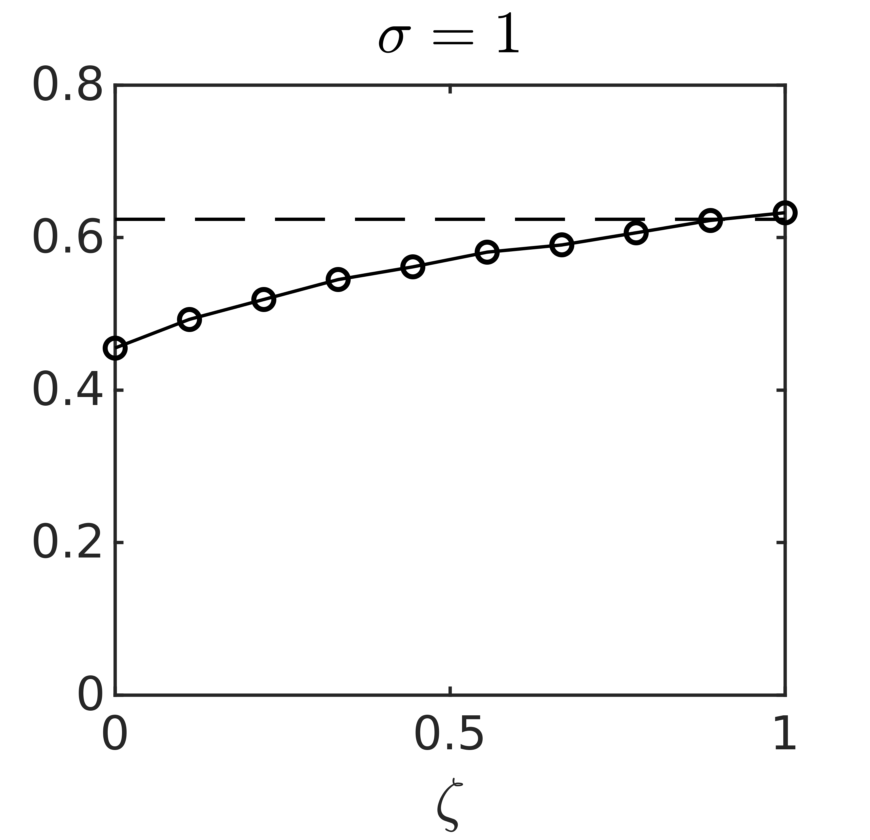
\includegraphics[scale=0.9]{Figures/OUSubs_s10}
		\end{tabular}
		\end{figure}
	
		\BR{Issue}: How do we choose $\zeta \in (0, 1)$?
	}
\end{frame}

\begin{frame}
\frametitle{Filtering the data\footnote{\cite{AGP20}}}
	
	\NB{Idea}: Consider
	\begin{equation}
		Z^\epl_t = \int_0^t k(t,s) X^\epl_s \dd s,
	\end{equation}
	
	\begin{overlayarea}{\textwidth}{0.5\textheight}
	
	\only<1>{
		where $\delta, \beta > 0$ and 
		\begin{equation}
			k(t, s) = C_\beta \delta^{-1/\beta} e^{-\frac1\delta (t-s)^\beta}, \qquad C_\beta = \beta \, \Gamma(1/\beta)^{-1}.
		\end{equation}
	
		\BR{Why?} Subsampling data is a ``smoothing'' process, so why not directly smoothing the data?
	}
	
	\only<2-3>{
		where $\delta > 0$ and ($\beta = 1$)
		\begin{equation}
			k(t, s) = \delta^{-1} e^{-\frac1\delta (t-s)}.
		\end{equation}
	}
	
	\only<2>{
		We can write
		\begin{equation}
			\d Z^\epl_t = k(t,t) X^\epl_t \dd t + \int_0^t \partial_t k(t,s) X^\epl_s \dd s \dd t = \frac{1}{\delta} \left ( X^\epl_t - Z^\epl_t \right ) \dd t.
		\end{equation}
	}
	
	\only<3>{
		We can write
		\begin{equation}
		\begin{aligned}
			\d X_t^\epl &= -\alpha \cdot V'(X_t^\epl) \dd t - \frac1\epl p'\left(\frac{X_t^\epl}\epl\right) \dd t+ \sqrt{2\sigma} \dd W_t, \\
			\d Z^\epl_t &= \frac1\delta\left( X^\epl_t - Z^\epl_t \right) \dd t. \qquad \to \FG{\text{System of coupled SDEs!}}
		\end{aligned}
		\end{equation}
	}
	\end{overlayarea}
\end{frame}

\begin{frame}
\frametitle{Ergodic properties of the filter}

	\only<1> {
		\NB{Now:} Something we can work on
		\begin{equation}
		\begin{aligned}
			\d X_t^\epl &= -\alpha \cdot V'(X_t^\epl) \dd t - \frac1\epl p'\left(\frac{X_t^\epl}\epl\right) \dd t+ \sqrt{2\sigma} \dd W_t, \\
			\d Z^\epl_t &= \frac1\delta\left( X^\epl_t - Z^\epl_t \right) \dd t.
		\end{aligned}
		\end{equation}
		
		\BR{We have} $(X^\epl_t, Z^\epl_t)^\top$ geometrically ergodic with smooth invariant density.
		 
		\FG{Invariant measure} $\mu^\epl(\d x, \d z) = \rho^\epl(x, z) \dd x \dd z$ satisfies stationary FP
		\begin{equation}
		\begin{aligned}
		\sigma \partial^2_{xx} \rho^\epl(x,z) &+ \partial_x\left(\left(\alpha \cdot V'(x) + \frac{1}\epl p' \left ( \frac{x}\epl \right ) \right) \rho^\epl(x,z)\right) \\
		&+ \frac{1}{\delta} \partial_z\left((z - x) \rho^\epl(x,z)\right)= 0.
		\end{aligned}
		\end{equation}
	}

	\only<2> {
		\begin{lemma}\label{lem:FPMarginal} Let us write $\rho^\epl(x, z) = \phi^\epl(x)\psi^\epl(z)R^\epl(x,z),$ with $\phi^\epl$, $\psi^\epl$ marginal densities wrt $x$ and $z$. Then, it holds
		\begin{equation}\label{eq:marginalX}
			\phi^\epl(x) = \frac{1}{C_{\phi^\epl}} \exp\left(-\frac{1}{\sigma} \alpha \cdot V(x) - \frac{1}{\sigma} p \left ( \frac{x}\epl \right )\right),
		\end{equation}
		Moreover, the ``magic equality'' holds
		\begin{equation}
			\sigma \delta \int_{\R} \int_{\R} V'(z) \phi^\epl(x) \psi^\epl(z) \partial_x R^\epl(x,z) \dd x \dd z = \E^{\rho^\epl}[((X^\epl)^2 - (Z^\epl)^2)V''(Z^\epl)].
		\end{equation}
		\end{lemma}
		
		\vspace{0.3cm}
		\BR{Remark}: $\phi^\epl = $ invariant measure of $X^\epl$ alone.
	}
	\only<3>{
		\NB{Question:} What happens in the limit $\epl \to 0$?
		
		\vspace{0.5cm}	
		\begin{lemma} The measure $\mu^\epl$ converges weakly to $\mu^0(\d x, \d z) = \rho^0(x, z) \dd x \dd z$ satisfying
		\begin{equation}
			\Sigma \partial^2_{xx} \rho^0(x,z) +  \partial_x\left(A \cdot V'(x)  \rho^0(x,z)\right) +\frac1\delta \partial_z \left((z - x) \rho^0(x,z)\right) = 0,
		\end{equation}
		where $A$ and $\Sigma$ coefficients of the homogenized equation.
		\end{lemma}
	}
\end{frame}

\begin{frame}
	\frametitle{Back to parameter estimation}
	
	\NB{Estimator}:
	\begin{equation}
		\widehat A^\epl(T) = - \frac{\int_0^T V'(X^\epl_t) \dd X^\epl_t}{\int_0^T V'(X^\epl_t)^2 \dd t}.
	\end{equation}
	
	\NB{Idea}: Replace $X_t^\epl$ with $Z_t^\epl$ (but not everywhere)
	\begin{equation}
		\widehat A^\epl_Z(T) = - \frac{\int_0^T V'(Z^\epl_t) \dd X^\epl_t}{\int_0^T V'(Z^\epl_t) V'(X^\epl_t) \dd t}.
	\end{equation}	
	\begin{overlayarea}{\textwidth}{0.3\textheight}
		\only<1>{
			\BR{Remark}: Denominator $\neq$ 0 a.s. $\implies \widehat A^\epl_Z(T)$ well-defined.
		}
		\only<2>{
			\begin{theorem}
				\begin{equation}
					\lim_{\epl \to 0} \lim_{T \to \infty} \widehat A_Z^\epl(T) = A, \quad \text{a.s.},
				\end{equation}
				where $A$ drift coefficient of homogenized equation.
			\end{theorem}
			\BR{Remark}: True also for $N$ parameters and $d$-dimensional SDE.
		}
	\end{overlayarea}
\end{frame}

\begin{frame}
	\frametitle{Back to parameter estimation}
	\NB{Result}:
	\begin{equation}
		\lim_{\epl \to 0} \lim_{T \to \infty} \widehat A^\epl(T) = - \lim_{\epl \to 0} \lim_{T \to \infty} \frac{\int_0^T V'(Z^\epl_t) \dd X^\epl_t}{\int_0^T V'(Z^\epl_t)V'(X^\epl_t) \dd t} = A, \quad \text{a.s.}
	\end{equation}
	
	\BR{Proof steps}:
	
	\vspace{0.2cm}
	\begin{overlayarea}{\textwidth}{0.5\textheight}
	\only<1>{
		Replace $\d X_t^\epl$ in the estimator
		\begin{equation}
		\begin{alignedat}{2}
			-\frac{\int_0^T V'(X^\epl_t) \dd X^\epl_t}{\int_0^T V'(Z^\epl_t) V'(X^\epl_t)\dd t} &= \alpha\frac{\int_0^T V'(Z^\epl_t) V'(X^\epl_t) \dd t}{\int_0^T V'(Z^\epl_t) V'(X^\epl_t) \dd t} &&\quad = \alpha \\
			&+ \frac1\epl \frac{\int_0^T V'(Z^\epl_t)  p'\left(\frac{X^\epl_t}{\epl}\right) \dd t}{\int_0^T V'(Z^\epl_t)V'(X^\epl_t) \dd t} &&\quad \eqqcolon I_1^\epl(T) \\
			&- \sqrt{2\sigma}\frac{\int_0^T V'(Z^\epl_t) \dd W_t}{\int_0^T V'(Z^\epl_t) V'(X^\epl_t) \dd t} &&\quad \eqqcolon I_2^\epl(T)
		\end{alignedat}
		\end{equation}
	}
	\only<2>{
		Take care of the first remainder
		\begin{equation}
			 \lim_{\epl \to 0} \lim_{T \to \infty} I_2^\epl(T) = \lim_{\epl \to 0} \lim_{T \to \infty} \sqrt{2\sigma}\frac{\int_0^T V'(Z^\epl_t) \dd W_t}{\int_0^T V'(Z^\epl_t)V'(X^\epl_t) \dd t} = 0, \quad \text{a.s.},
		\end{equation}
		due to the strong LLN for (continuous) martingales.	
	}
	\only<3>{
		Take care of the second ``remainder''
		\begin{equation}
			\lim_{\epl \to 0} \lim_{T \to \infty} I_1^\epl(T) = \lim_{\epl \to 0} \lim_{T \to \infty} \frac1\epl \frac{\int_0^T V'(Z^\epl_t)  p'\left(\frac{X^\epl_t}{\epl}\right) \dd t}{\int_0^T V'(Z^\epl_t)V'(X^\epl_t) \dd t} = A - \alpha, \quad \text{a.s.},
		\end{equation}
		applying 
		\begin{enumerate}
			\item ergodic theorem for $T \to \infty$ and ``magic equality''
			\item convergence $\mu^\epl \to \mu^0$ for $\epl \to 0$ and ``magic equality'' again
		\end{enumerate}
	}
	\end{overlayarea}
\end{frame}

\begin{frame}
	\frametitle{Numerical experiments}
	
	\only<1> {
		\BR{Reminder}: Filter had a parameter $\beta$:
		\begin{equation}
			k(t, s) = C_\beta \delta^{-1/\beta} e^{-\frac1\delta (t-s)^\beta}, \qquad C_\beta = \beta \, \Gamma(1/\beta)^{-1}.
		\end{equation}
		We did analysis for $\beta = 1$ but show experiments for larger values of $\beta$, too.
		
	}
	
	\only<2> {
		\BR{Setting}: Estimate $A$ for $V(x) = x^2/2$ (Ornstein--Uhlenbeck) with subsampling varying $\delta = \epl^\zeta$ ($\epl = 0.1$, $T = 10^3$, $p(y) = \cos(y)$)
		
		\vspace{0.3cm}
		\begin{figure}
			\begin{tabular}{ccc}
				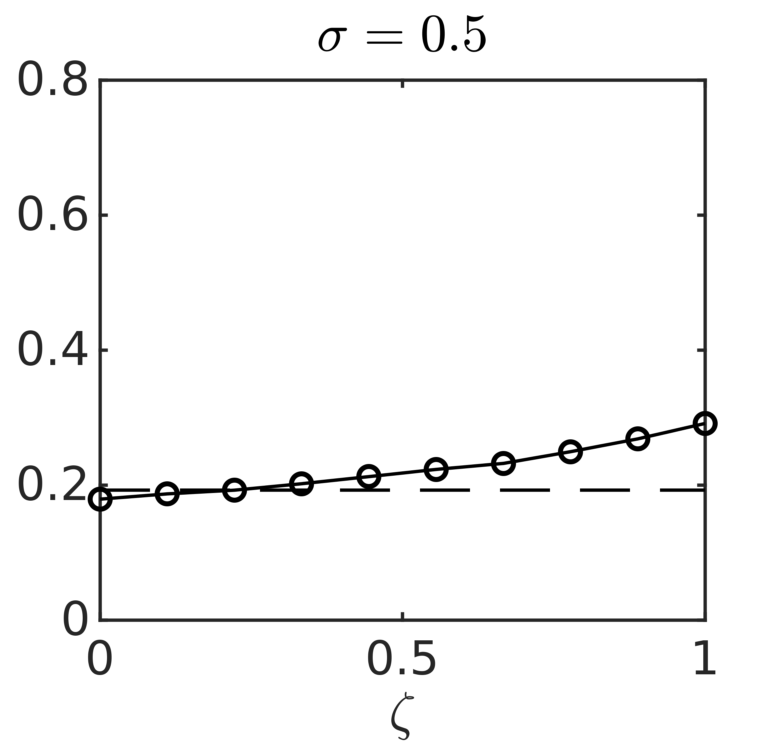
\includegraphics[scale=0.85]{Figures/OUSubs_s5} & 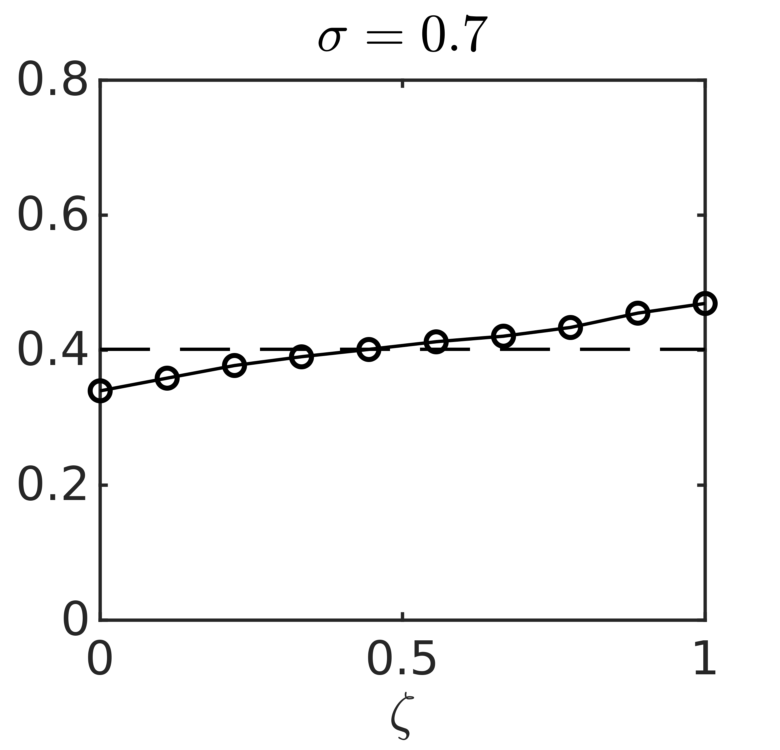
\includegraphics[scale=0.85]{Figures/OUSubs_s7} & 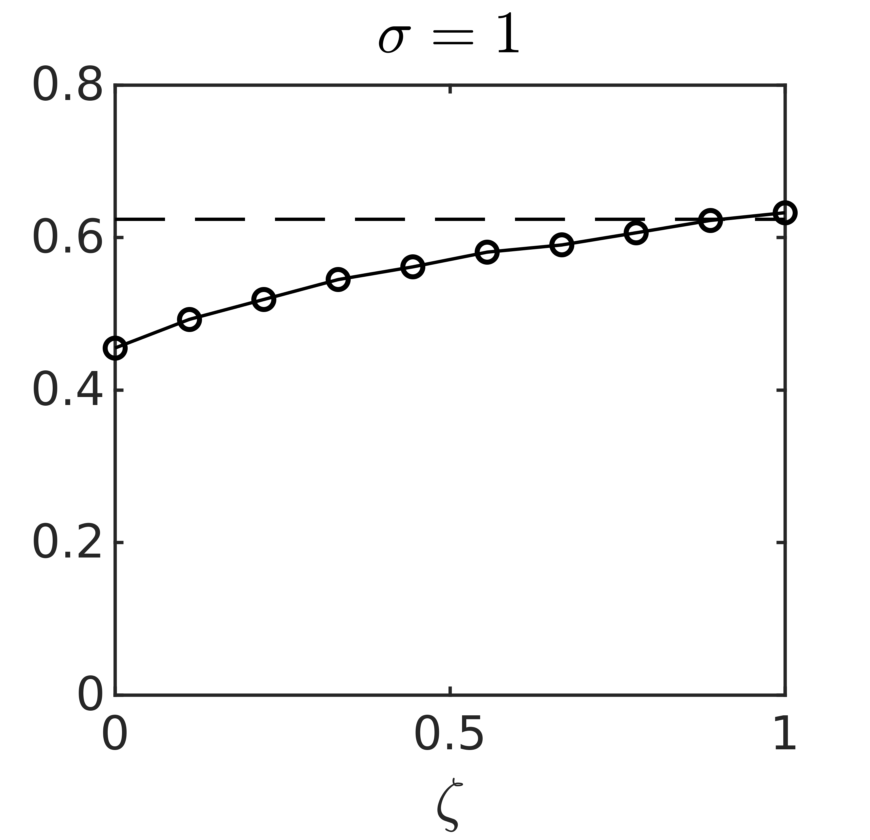
\includegraphics[scale=0.85]{Figures/OUSubs_s10}
			\end{tabular}
		\end{figure}
		
		\BR{Issue}: How do we pick $\zeta \in (0, 1)$?			
	}
	
	\only<3> {
		\BR{Setting}: Estimate $A$ for $V(x) = x^2/2$ (Ornstein--Uhlenbeck) with filtering \FG{$\beta = 1$} and $\delta = \epl^\zeta$ ($\epl = 0.1$, $T = 10^3$, $p(y) = \cos(y)$)
		
		\vspace{0.3cm}
		\begin{figure}
			\begin{tabular}{ccc}
				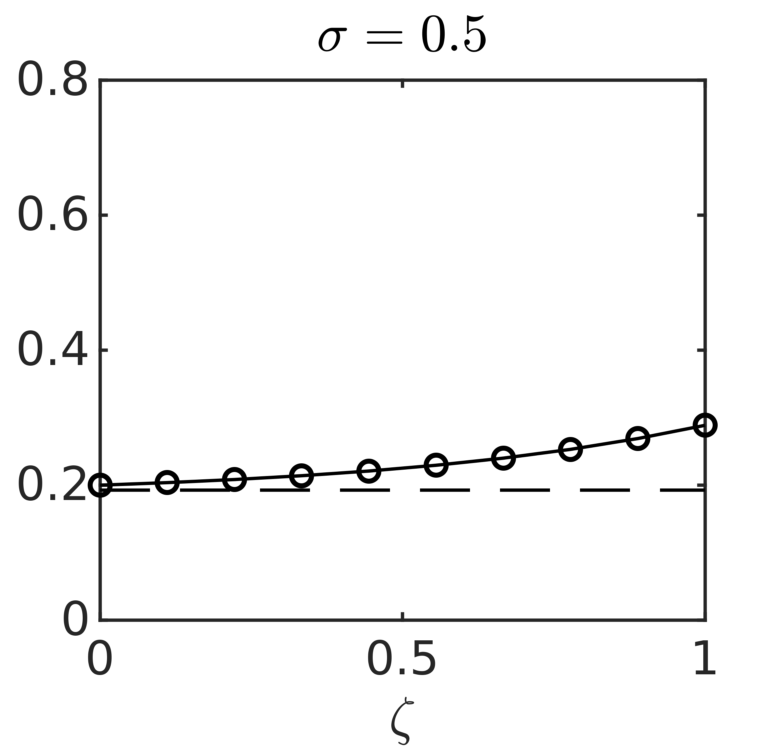
\includegraphics[scale=0.85]{Figures/OUFilt_s5_b1} & 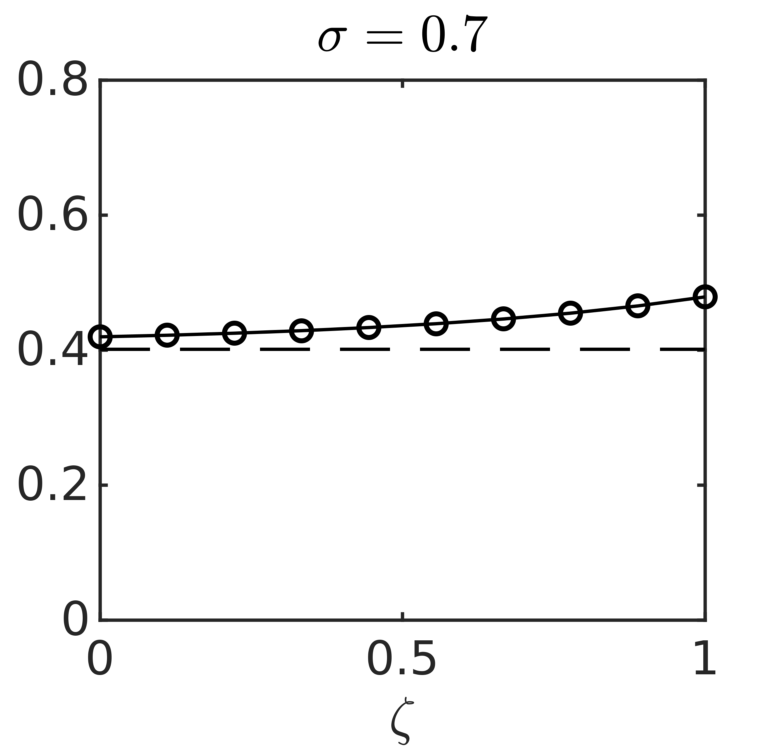
\includegraphics[scale=0.85]{Figures/OUFilt_s7_b1} & 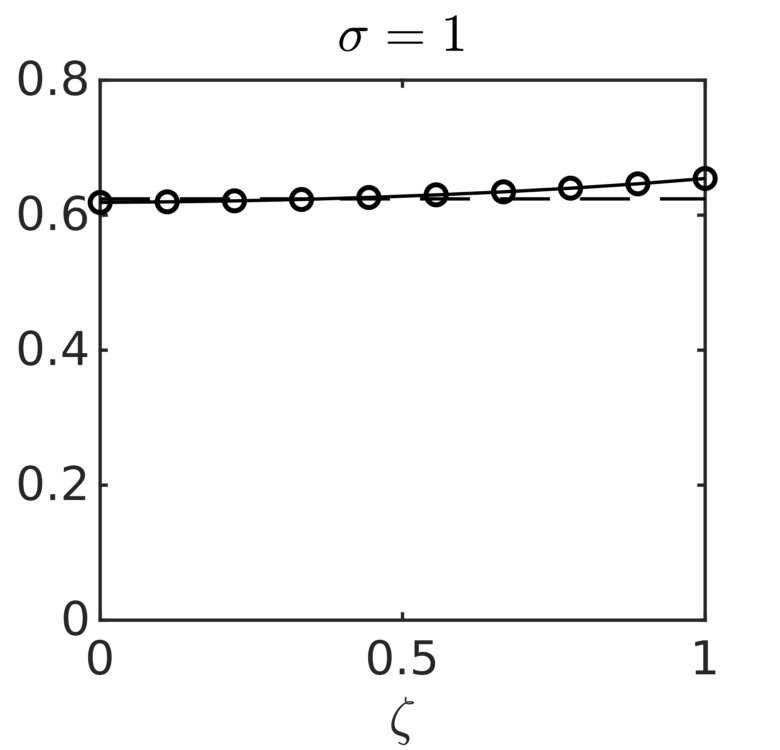
\includegraphics[scale=0.85]{Figures/OUFilt_s10_b1}
			\end{tabular}
		\end{figure}
		
		\BR{Remark}: Results still depend on $\delta$ - less than subsampling
	}
	
	\only<4> {
		\BR{Setting}: Estimate $A$ for $V(x) = x^2/2$ (Ornstein--Uhlenbeck) with filtering \FG{$\beta = 5$} and $\delta = \epl^\zeta$ ($\epl = 0.1$, $T = 10^3$, $p(y) = \cos(y)$)
	
		\vspace{0.3cm}
		\begin{figure}
			\begin{tabular}{ccc}
				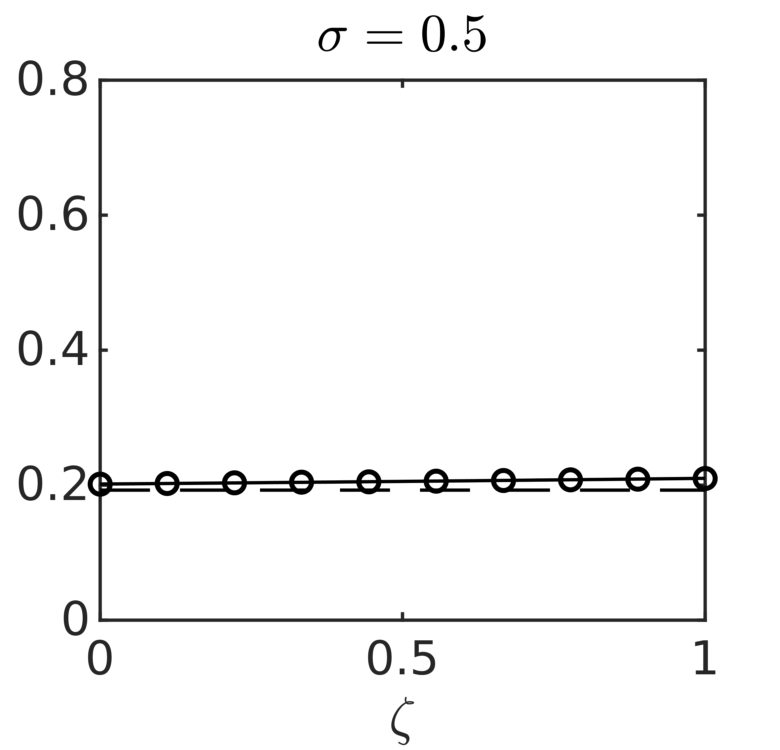
\includegraphics[scale=0.85]{Figures/OUFilt_s5_b5} & 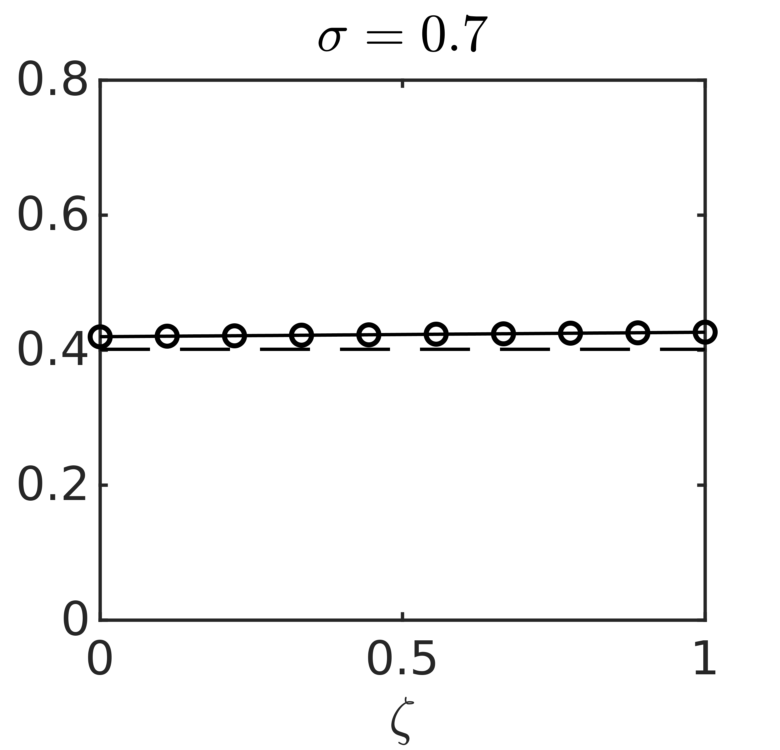
\includegraphics[scale=0.85]{Figures/OUFilt_s7_b5} & 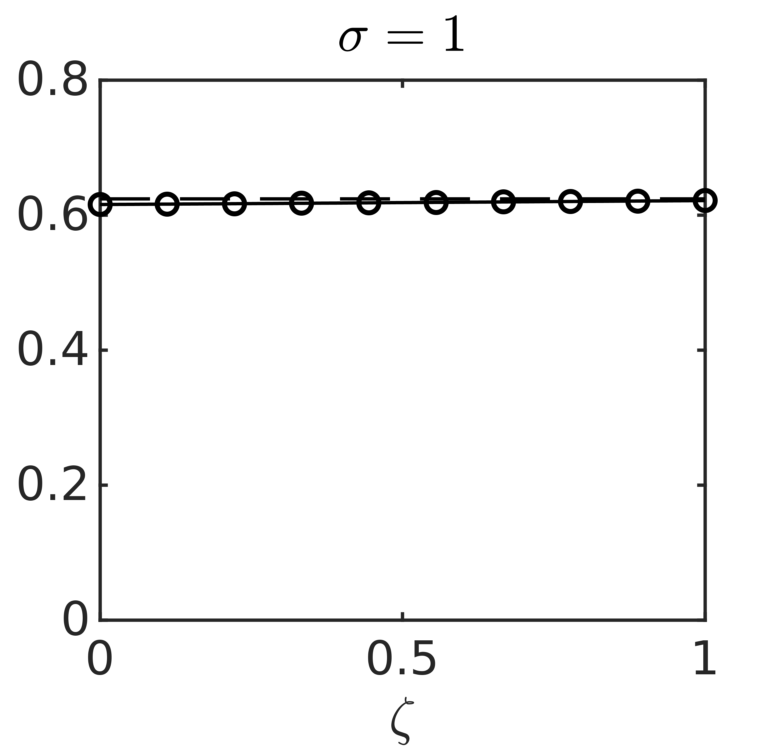
\includegraphics[scale=0.85]{Figures/OUFilt_s10_b5}
			\end{tabular}
		\end{figure}
		
		\BR{Remark}: Dependence on $\delta$ disappeared
	}
	
	\only<5> {
		\BR{Setting}: Estimate $A$ for $V(x) = x^2/2$ (Ornstein--Uhlenbeck) with filtering \FG{variable $\beta$} and $\delta$ fixed ($\epl = 0.1$, $T = 10^3$, $p(y) = \cos(y)$)
		
		\vspace{0.3cm}
		\begin{figure}
			\begin{tabular}{ccc}
				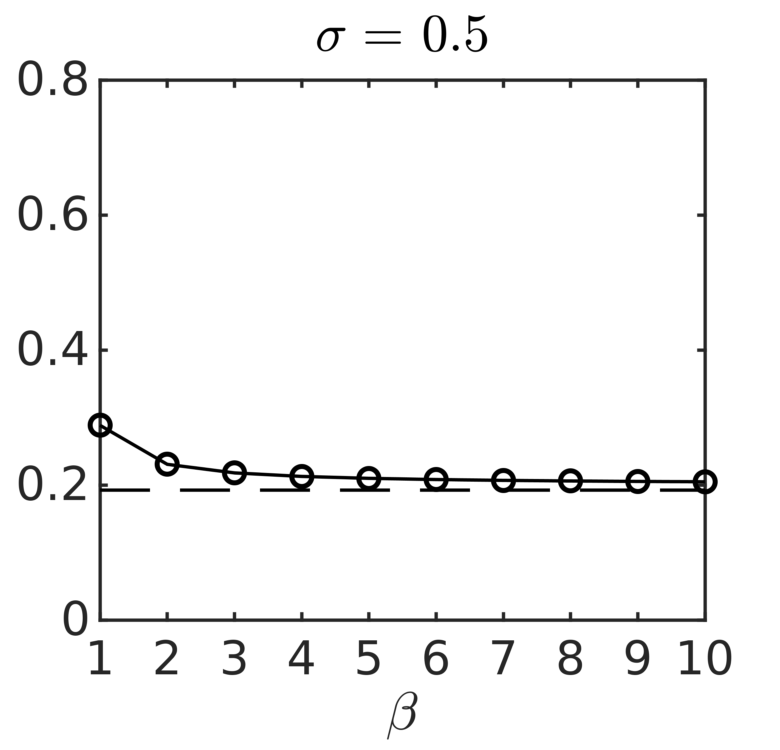
\includegraphics[scale=0.85]{Figures/OUBeta_s5} & 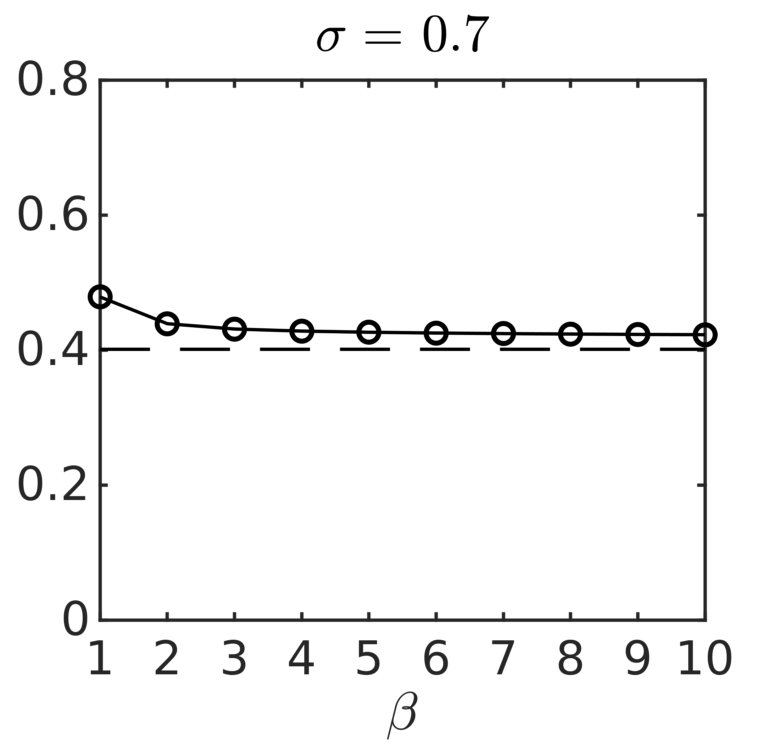
\includegraphics[scale=0.85]{Figures/OUBeta_s7} & 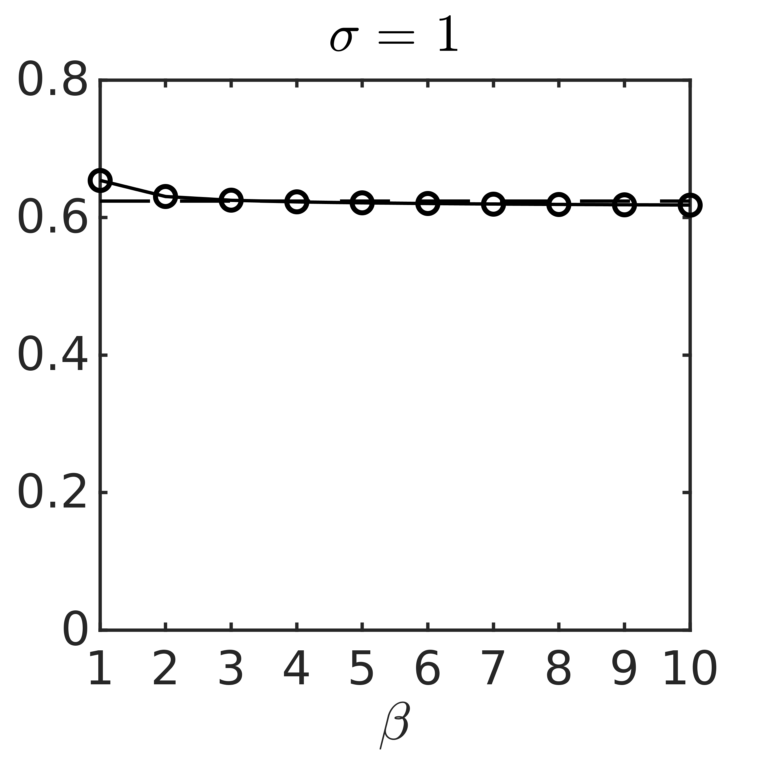
\includegraphics[scale=0.85]{Figures/OUBeta_s10}
			\end{tabular}
		\end{figure}
		
		\BR{Remark}: Results stabilize fast wrt $\beta$
	}
	
	\only<6> {
		\BR{Setting}: Estimate $A \in \R^4$ for $V_i(x) = x^{2i}/(2i)$, $i = 1, \ldots, 4$ with, no pre-processing, subsampling and filtering \FG{$\beta = 1$} ($\epl = 0.05$, $T = 10^3$, $p(y) = \cos(y)$)
		
		\vspace{0.3cm}
		\begin{figure}
			\begin{tabular}{ccc}
				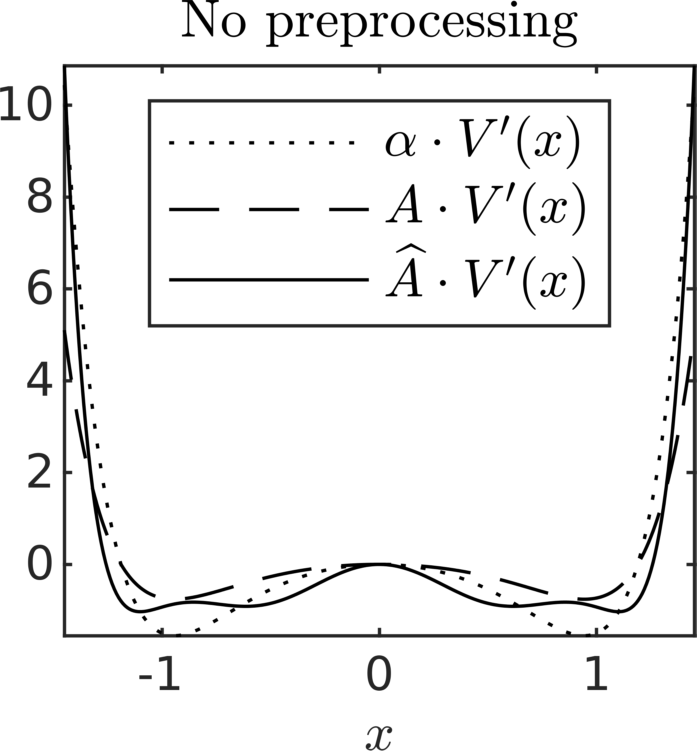
\includegraphics[scale=0.9]{Figures/KLNothing} & 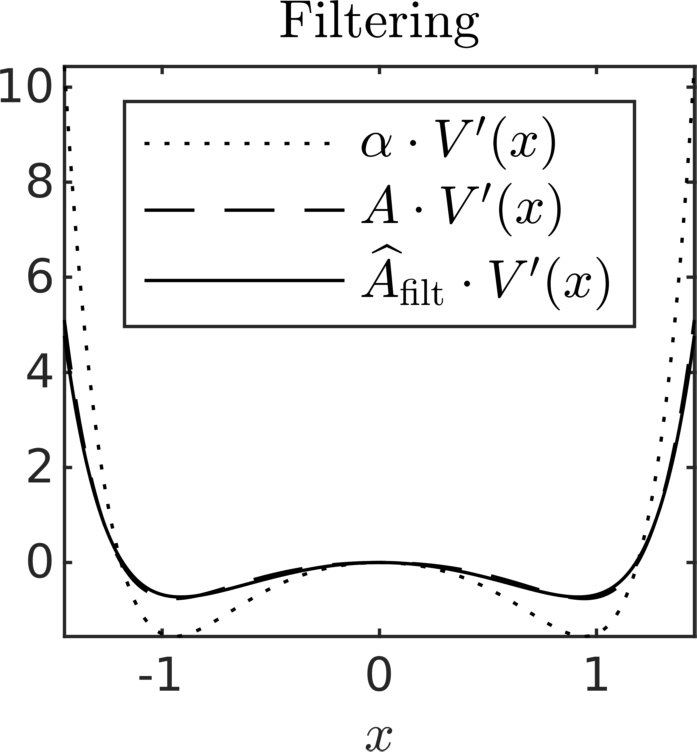
\includegraphics[scale=0.9]{Figures/KLFilt} & 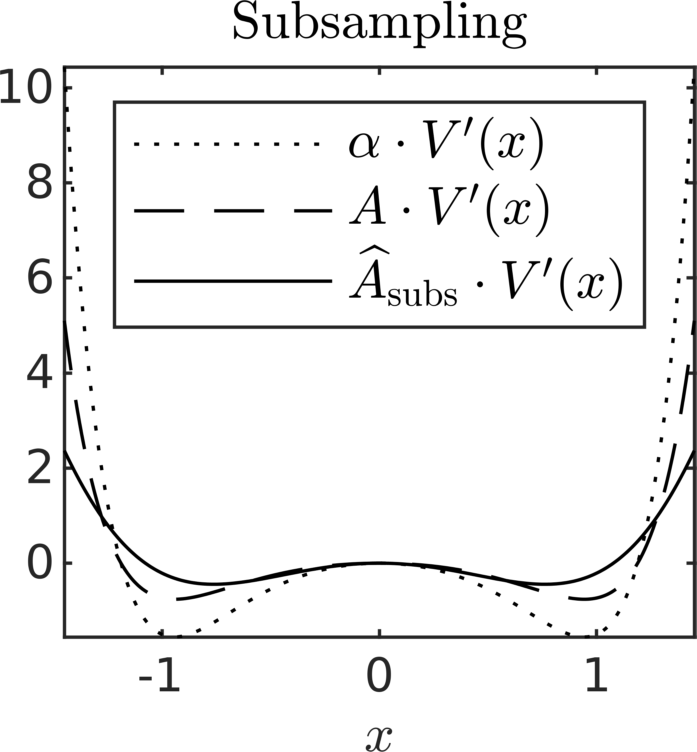
\includegraphics[scale=0.9]{Figures/KLSubs}
			\end{tabular}
		\end{figure}
		
		\BR{Remark}: Estimate with filter can be done in multi-dimensional case, too.
	}
\end{frame}

\begin{frame}
	\frametitle{The Bayesian paradigm}
	
	\only<1-2>{
		\vspace{0.6cm}
		\NB{A step back}: Likelihood function
		\begin{align}
			L(X^\epl \mid A) &= \exp\left(-\frac{I(X^\epl \mid A)}{2\Sigma}\right), \\
			I(X^\epl \mid A) &= \int_0^T A \cdot V'(X^\epl_t) \dd X^\epl_t + \frac12 \int_0^T \left( A \cdot V'(X^\epl_t) \right)^2 \dd t.
		\end{align}
		$\implies \log L(X^\epl \mid A)$}
	\only<1>{quadratic function of $A$.}\only<2>{\BR{quadratic function of $A$}.}
		
	\only<1-2>{
		\vspace{0.4cm}
		\NB{Prior}: Fix $\mu_0 = \mathcal N(A_0, C_0)$ on $A$, density $p_0$
		
		\vspace{0.4cm}
		\NB{Posterior}: Bayes' rule gives (densities)
	}
	\only<1>{
		\begin{equation}
			p(A \mid X^\epl) = \frac1Z \, L(X^\epl \mid A) \, p_0(A), 
		\end{equation}}
	\only<2>{
		\begin{equation}
		p(A \mid X^\epl) = \frac1Z \, L(X^\epl \mid A) \, p_0(A), \BR{\implies \text{Gaussian!}}
		\end{equation}
	}
	\only<3-4>{
		\NB{Posterior}: $\mu=\mathcal N(m_T, C_T)$ with (complete the squares)
		\begin{equation}
		\begin{aligned}
			C_T^{-1} &= C_0^{-1} + T M, \\
			C_T^{-1}m_T &= C_0^{-1}A_0 - T h,
		\end{aligned}
		\end{equation}
		where
		\begin{equation}
			M = \frac1{2\Sigma T}\int_0^T V'(X^\epl_t) \otimes V'(X^\epl_t) \dd t, \quad h = \frac1{2\Sigma T}\int_0^T V'(X^\epl_t) \dd X^\epl_t.
		\end{equation}
	}
	
	\only<3>{
		\vspace{0.3cm}
		\BR{Issue 1}: $\Sigma$ unknown -- estimate with e.g. subsampling	
	}	
	\only<4>{
		\vspace{0.3cm}
		\BR{Issue 2}: $\mu$ collapses to MLE for $T \to \infty$  \BR{...But MLE is wrong ($\alpha$)}
	}
\end{frame}

\begin{frame}
\frametitle{The Bayesian paradigm -- filtering solution}
	\only<1->{
		\vspace{0.4cm}
		\BR{Issue 2}: $\mu$ collapses to MLE for $T \to \infty$  \BR{...But MLE is wrong ($\alpha$)}
	}

	\begin{overlayarea}{\textwidth}{0.8\textheight}
	\only<1>{
		
		\vspace{0.4cm}	
		\NB{Idea}: Use the filter as before 
		\begin{align}
			\widetilde L^\epl(X \mid A) &= \exp\left(-\frac{\widetilde I^\epl(X\mid A)}{2\Sigma} \right), \\
			\widetilde I^\epl(X\mid A) &= \int_0^T A \cdot V'(Z_t^\epl) \dd X_t^\epl + \frac12 \int_0^T \left( A \cdot V'(Z_t^\epl) \right) \left( A \cdot V'(X_t^\epl) \right) \dd t.
		\end{align}
	}
	\only<2>{
		
		\vspace{0.4cm}
		\NB{Posterior}: $\mu=\mathcal N(\widetilde m_T, \widetilde C_T)$ with (complete the squares)
		\begin{equation}
		\begin{aligned}
			\widetilde C_T^{-1} &= C_0^{-1} + T \widetilde M_S, \\
			\widetilde C_T^{-1} \widetilde m_T &= C_0^{-1}A_0 - T \widetilde h,
		\end{aligned}
		\end{equation}
		where
		\begin{equation}
			\widetilde M = \frac1{2\Sigma T}\int_0^T V'(Z^\epl_t) \otimes V'(X^\epl_t) \dd t, \quad \widetilde h = \frac1{2\Sigma T}\int_0^T V'(X^\epl_t) \dd X^\epl_t,
		\end{equation}
		and $\widetilde M_S = \left(\widetilde M + \widetilde M^\top\right)/2$ $\implies$ \FG{$\widetilde \mu$ collapses to $A$ wrt $T$}.
	}
	\end{overlayarea}
	
\end{frame}

\begin{frame}
	\frametitle{Numerical Experiment}
	
	\BR{Setting}: Bistable potential $V_1(x) = x^4/4$, $V_2(x) = -x^2/2$, $\alpha_1 = 1$, $\alpha_2= 2$. Filtering $\beta = 1$, $\delta = 0.2$ ($\sigma=0.8$, $\epl = 0.05$, $T = 800$, $p(y) = \cos(y)$)
	
	\begin{figure}
		\begin{tabular}{ccc}
			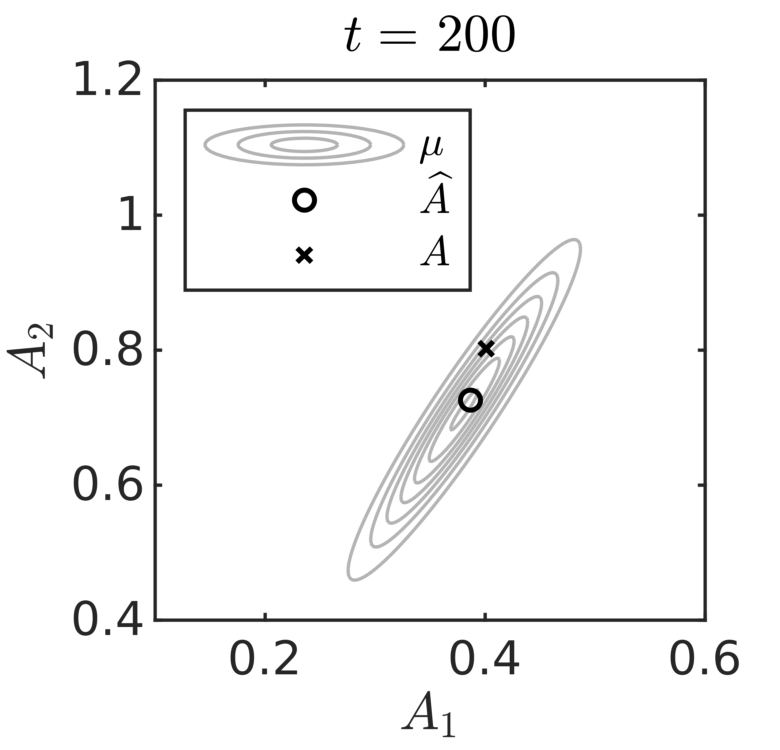
\includegraphics[scale=0.9]{Figures/Bayes_T200} & 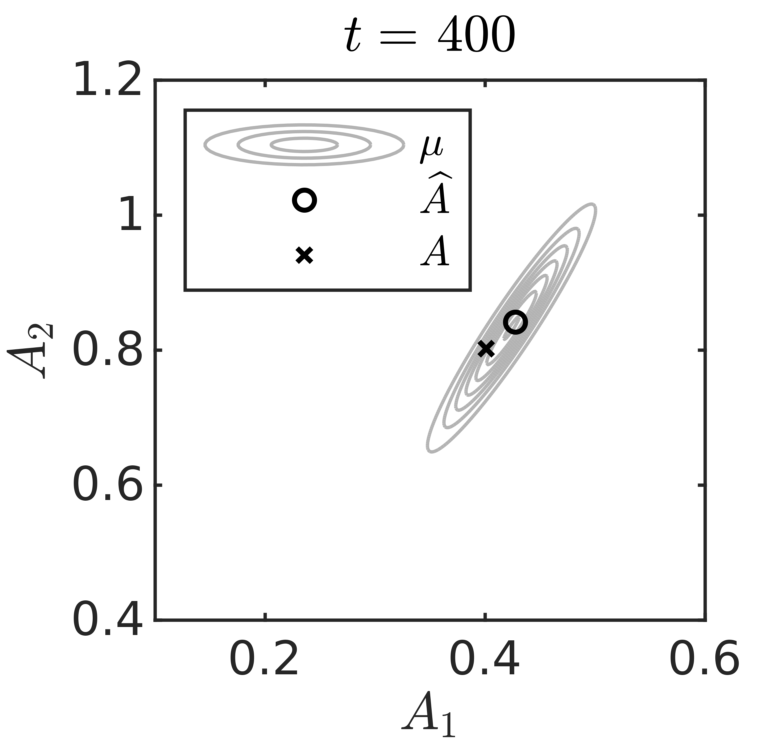
\includegraphics[scale=0.9]{Figures/Bayes_T400} & 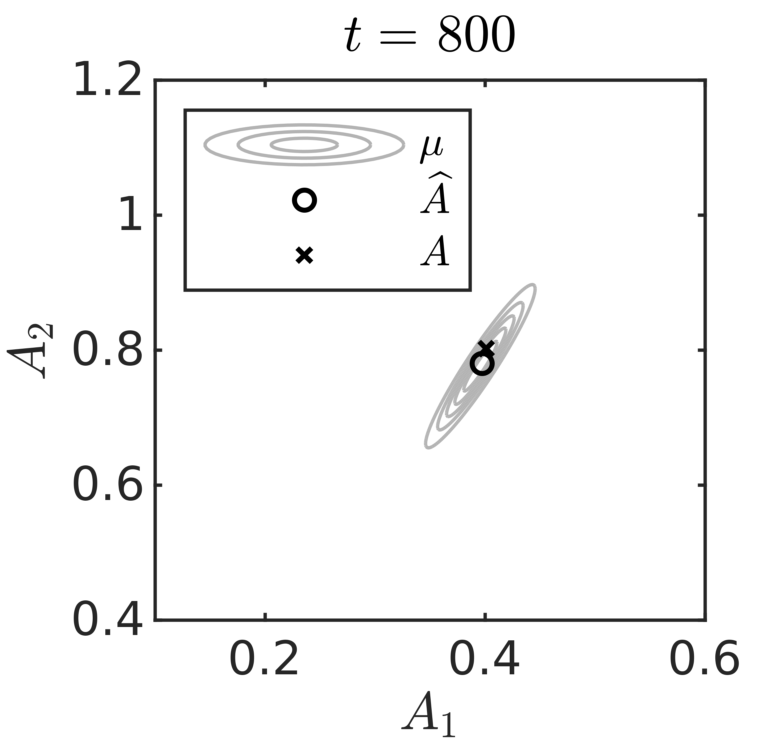
\includegraphics[scale=0.9]{Figures/Bayes_T800}
		\end{tabular}
	\end{figure}
	
	\BR{Remark}: As expected, posterior shrinks to MLE (and to $A$) wrt $t$
\end{frame}


\appendix
\begin{frame}[allowframebreaks]{References}

\bibliographystyle{apalike}
\begin{scriptsize}
	\bibliography{../anmc}
\end{scriptsize}

\end{frame}

\end{document}
